\documentclass[11pt,a4paper]{report}
\usepackage[textwidth=37em,vmargin=30mm]{geometry}
\usepackage{calc,xunicode,amsmath,amssymb,paralist,enumitem,tabu,booktabs,datetime2,xeCJK,xeCJKfntef,listings}
\usepackage{tocloft,fancyhdr,tcolorbox,xcolor,graphicx,eso-pic,xltxtra,xelatexemoji}

\newcommand{\envyear}[0]{2025}
\newcommand{\envdatestr}[0]{2025-03-30}
\newcommand{\envfinaldir}[0]{webdb/2025/20250330/final}

\usepackage[hidelinks]{hyperref}
\hypersetup{
    colorlinks=false,
    pdfpagemode=FullScreen,
    pdftitle={Web Digest - \envdatestr}
}

\setlength{\cftbeforechapskip}{10pt}
\renewcommand{\cftchapfont}{\rmfamily\bfseries\large\raggedright}
\setlength{\cftbeforesecskip}{2pt}
\renewcommand{\cftsecfont}{\sffamily\small\raggedright}

\setdefaultleftmargin{2em}{2em}{1em}{1em}{1em}{1em}

\usepackage{xeCJK,xeCJKfntef}
\xeCJKsetup{PunctStyle=plain,RubberPunctSkip=false,CJKglue=\strut\hskip 0pt plus 0.1em minus 0.05em,CJKecglue=\strut\hskip 0.22em plus 0.2em}
\XeTeXlinebreaklocale "zh"
\XeTeXlinebreakskip = 0pt


\setmainfont{Brygada 1918}
\setromanfont{Brygada 1918}
\setsansfont{IBM Plex Sans}
\setmonofont{JetBrains Mono NL}
\setCJKmainfont{Noto Serif CJK SC}
\setCJKromanfont{Noto Serif CJK SC}
\setCJKsansfont{Noto Sans CJK SC}
\setCJKmonofont{Noto Sans CJK SC}

\setlength{\parindent}{0pt}
\setlength{\parskip}{8pt}
\linespread{1.15}

\lstset{
	basicstyle=\ttfamily\footnotesize,
	numbersep=5pt,
	backgroundcolor=\color{black!5},
	showspaces=false,
	showstringspaces=false,
	showtabs=false,
	tabsize=2,
	captionpos=b,
	breaklines=true,
	breakatwhitespace=true,
	breakautoindent=true,
	linewidth=\textwidth
}






\newcommand{\coverpic}[2]{
    % argv: itemurl, authorname
    Cover photo by #2~~(\href{#1}{#1})
}
\newcommand{\makeheader}[0]{
    \begin{titlepage}
        % \newgeometry{hmargin=15mm,tmargin=21mm,bmargin=12mm}
        \begin{center}
            
            \rmfamily\scshape
            \fontspec{BaskervilleF}
            \fontspec{Old Standard}
            \fontsize{59pt}{70pt}\selectfont
            WEB\hfill DIGEST
            
            \vfill
            % \vskip 30pt
            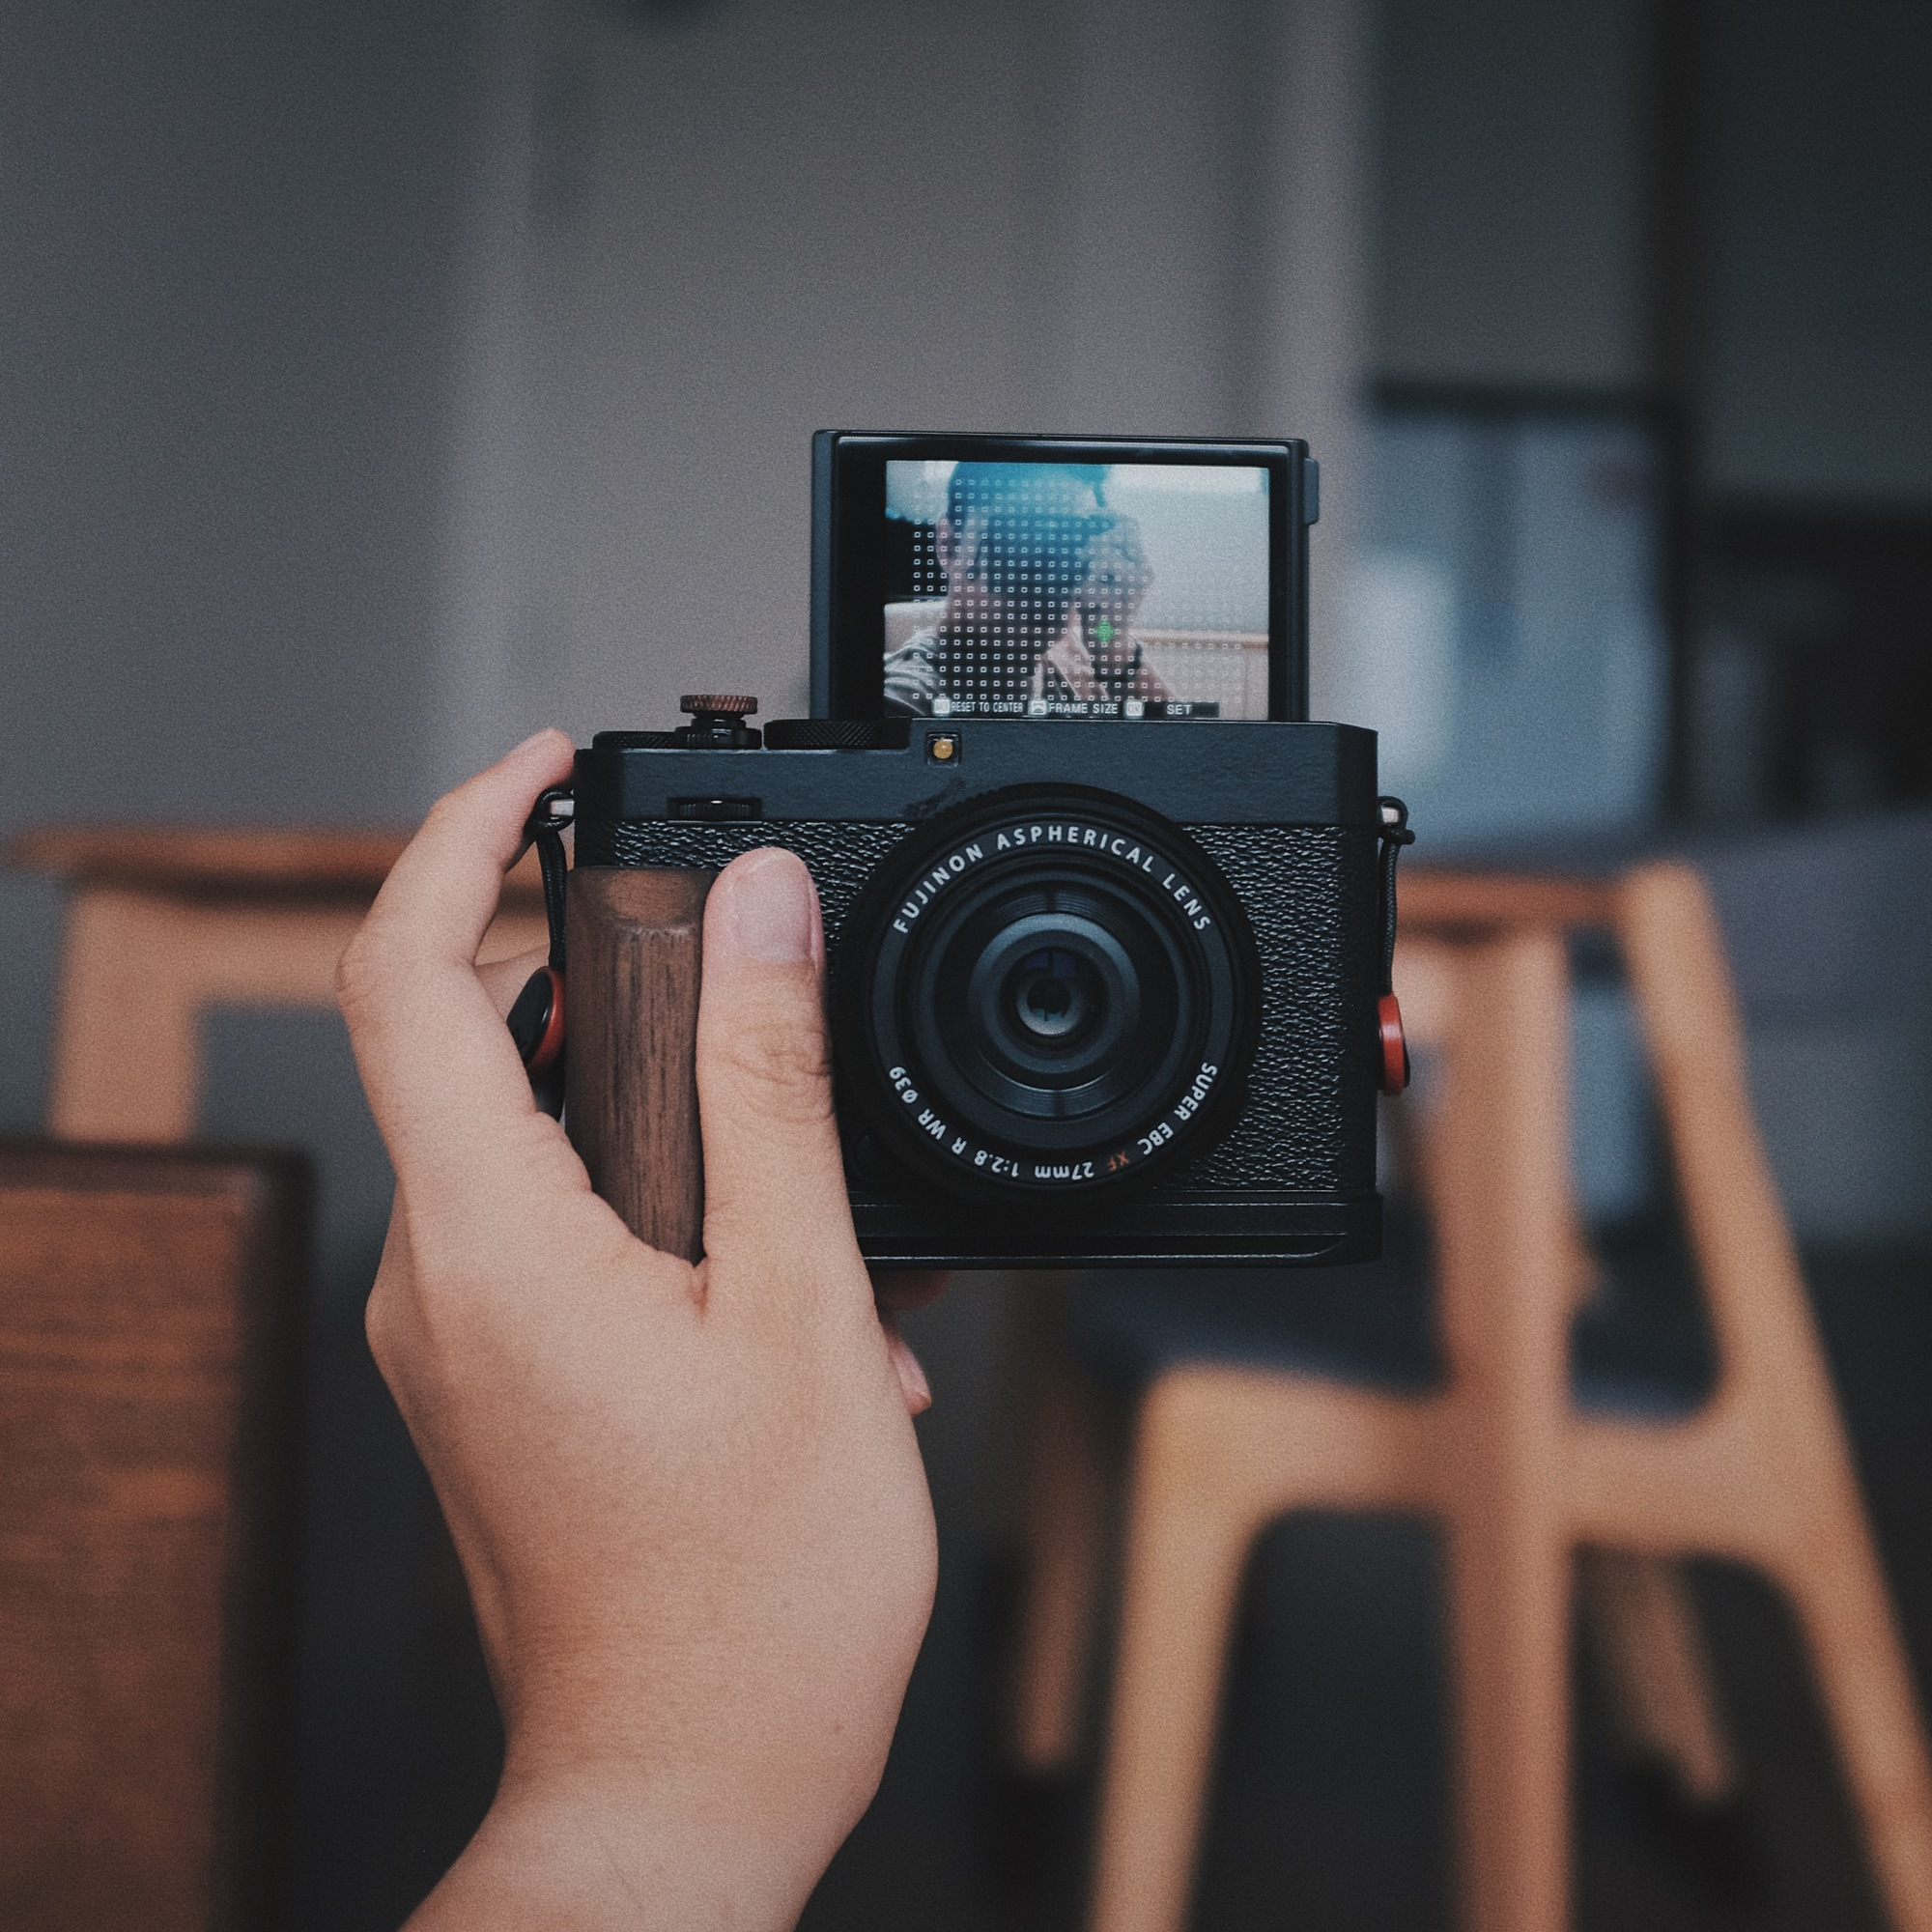
\includegraphics[width=\linewidth]{\envfinaldir/coverpic-prod.jpg}\par
            % \vskip 30pt
            \vfill

            \normalsize\rmfamily\scshape
            \copyright{} The Web Digest Project \hfill\large \envdatestr
        \end{center}
    \end{titlepage}
    % \restoregeometry
}
\newcommand{\simplehref}[1]{%
    \textcolor{blue!80!green}{\href{#1}{#1}}%
}
\renewcommand{\contentsname}{\center\Huge\sffamily\bfseries Contents\par\vskip 20pt}
\newcounter{ipartcounter}
\setcounter{ipartcounter}{0}
\newcommand{\ipart}[1]{
    % \vskip 20pt
    \clearpage
    \stepcounter{ipartcounter}
    \phantomsection
    \addcontentsline{toc}{chapter}{#1}
    % \begin{center}
    %     \Huge
    %     \sffamily\bfseries
    %     #1
    % \end{center}
    % \vskip 20pt plus 7pt
}
\newcounter{ichaptercounter}
\setcounter{ichaptercounter}{0}
\newcommand{\ichapter}[1]{
    % \vskip 20pt
    \clearpage
    \stepcounter{ichaptercounter}
    \phantomsection
    \addcontentsline{toc}{section}{\numberline{\arabic{ichaptercounter}}#1}
    \begin{center}
        \Huge
        \sffamily\bfseries
        #1
    \end{center}
    \vskip 20pt plus 7pt
}
\newcommand{\entrytitlefont}[1]{\subsection*{\raggedright\Large\sffamily\bfseries#1}}
\newcommand{\entryitemGeneric}[2]{
    % argv: title, url
    \parbox{\linewidth}{
        \entrytitlefont{#1}\par\vskip 5pt
        \footnotesize\ttfamily\mdseries
        \simplehref{#2}
    }\vskip 11pt plus 11pt minus 1pt
}
\newcommand{\entryitemGithub}[3]{
    % argv: title, url, desc
    \parbox{\linewidth}{
        \entrytitlefont{#1}\par\vskip 5pt
        \footnotesize\ttfamily\mdseries
        \simplehref{#2}\par\vskip 5pt
        \small\rmfamily\mdseries#3
    }\vskip 11pt plus 11pt minus 1pt
}
\newcommand{\entryitemAp}[3]{
    % argv: title, url, desc
    \parbox{\linewidth}{
        \entrytitlefont{#1}\par\vskip 5pt
        \footnotesize\ttfamily\mdseries
        \simplehref{#2}\par\vskip 5pt
        \small\rmfamily\mdseries#3
    }\vskip 11pt plus 11pt minus 1pt
}
\newcommand{\entryitemHackernews}[3]{
    % argv: title, hnurl, rawurl
    % \parbox{\linewidth}{
    %     \entrytitlefont{#1}\par\vskip 5pt
    %     \footnotesize\ttfamily\mdseries
    %     \simplehref{#3}\par
    %     \textcolor{black!50}{\href{#2}{#2}}
    % }\vskip 11pt plus 11pt minus 1pt
    \begin{minipage}{\linewidth}
            \entrytitlefont{#1}\par\vskip 5pt
            \footnotesize\ttfamily\mdseries
            \simplehref{#3}\par
            \textcolor{black!50}{\href{#2}{#2}}
    \end{minipage}\par\vskip 11pt plus 11pt minus 1pt
}







\begin{document}

\makeheader

\tableofcontents\clearpage




\ipart{Developers}
\ichapter{Hacker News}
\entryitemTwoLinks{Apple's AI isn't a letdown. AI is the letdown}{https://news.ycombinator.com/item?id=43518576}{https://www.cnn.com/2025/03/27/tech/apple-ai-artificial-intelligence/index.html}

\entryitemTwoLinks{When the physicists need burner phones, that's when you know America's changed}{https://news.ycombinator.com/item?id=43517590}{https://www.theguardian.com/us-news/2025/mar/29/when-the-physicists-need-burner-phones-thats-when-you-know-americas-changed}

\entryitemTwoLinks{Paged Out \#6 is out}{https://news.ycombinator.com/item?id=43517375}{https://pagedout.institute/?page=blog.php\#entry-2025-03-29}

\entryitemTwoLinks{Veloren – voxel action-adventure role-playing in Rust}{https://news.ycombinator.com/item?id=43517337}{https://veloren.net/}

\entryitemTwoLinks{Why Apple's Severance gets edited over remote desktop software}{https://news.ycombinator.com/item?id=43517301}{https://tedium.co/2025/03/29/severance-apple-remote-editing-weirdness/}

\entryitemTwoLinks{Accessible open textbooks in math-heavy disciplines}{https://news.ycombinator.com/item?id=43516733}{https://richardzach.org/2025/03/accessible-open-textbooks-in-math-heavy-disciplines/}

\entryitemTwoLinks{Why I'm No Longer Talking to Architects About Microservices}{https://news.ycombinator.com/item?id=43515563}{https://blog.container-solutions.com/why-im-no-longer-talking-to-architects-about-microservices}

\entryitemTwoLinks{Koto Programming Language}{https://news.ycombinator.com/item?id=43514915}{https://koto.dev/}

\entryitemTwoLinks{Real Time Chess – A physical chess board without the concept of turns}{https://news.ycombinator.com/item?id=43514695}{https://github.com/misprit7/real-time-chess}

\entryitemTwoLinks{Show HN: Physical Pomodoro Timer with ESP32 and e-paper screen}{https://news.ycombinator.com/item?id=43514383}{https://github.com/Rukenshia/pomodoro}

\entryitemTwoLinks{Et Tu, Grammarly?}{https://news.ycombinator.com/item?id=43514308}{https://dbushell.com/2025/03/29/et-tu-grammarly/}

\entryitemTwoLinks{Today Google bricked my Chromebook by force-installing a hidden extension}{https://news.ycombinator.com/item?id=43514087}{https://cloudisland.nz/@rmi/114219847307106213}

\entryitemTwoLinks{Postgres Language Server: Initial Release}{https://news.ycombinator.com/item?id=43513996}{https://github.com/supabase-community/postgres-language-server}

\entryitemTwoLinks{Trump's attacks on universities get darker, with shadows reaching our shores}{https://news.ycombinator.com/item?id=43513811}{https://christinapagel.substack.com/p/trumps-attacks-on-universities-get}

\entryitemTwoLinks{Upcoming Windows 11 builds cannot install without internet and Microsoft Account}{https://news.ycombinator.com/item?id=43512660}{https://infosec.exchange/@wdormann/114242475168860209}

\entryitemTwoLinks{Plain – a web framework for building products with Python}{https://news.ycombinator.com/item?id=43512589}{https://plainframework.com/}

\entryitemTwoLinks{OpenWrt Two Approval}{https://news.ycombinator.com/item?id=43512495}{https://openwrt.org/voting/2025-02-12-openwrt-two}

\entryitemTwoLinks{iCloud Mail has DNS misconfigured?}{https://news.ycombinator.com/item?id=43511464}{https://www.mail-tester.com/test-p3tdhnk3o}

\entryitemTwoLinks{Madison Square Garden's surveillance banned this fan over his T-shirt design}{https://news.ycombinator.com/item?id=43511340}{https://www.theverge.com/news/637228/madison-square-garden-james-dolan-facial-recognition-fan-ban}

\entryitemTwoLinks{Windows 11 is closing a loophole that let you skip making a Microsoft account}{https://news.ycombinator.com/item?id=43511073}{https://www.theverge.com/news/638967/microsoft-windows-11-account-internet-bypass-blocked}\ichapter{Phoronix}
\entryitemGeneric{\hskip 0pt{}Intel's 2025-Q1 Linux Excitement With Battlemage, AVX10 \& Other Kernel Improvements}{https://www.phoronix.com/news/Intel-Linux-2025-Q1-Recap}

\entryitemGeneric{\hskip 0pt{}Firmware Loader Makes It Possible To Use Old Samsung TV Cameras On Linux}{https://www.phoronix.com/news/Samsung-TV-Cameras-Linux}

\entryitemGeneric{\hskip 0pt{}Linux 6.15 PCI Brings New Drivers For Agilex PCIe Controller \& AMD Multimedia DMA Bridge}{https://www.phoronix.com/news/Linux-6.15-PCI}

\entryitemGeneric{\hskip 0pt{}Xiph.Org's Theora libtheora 1.2 Officially Released: 16 Years After v1.0}{https://www.phoronix.com/news/Theora-1.2-Released}

\entryitemGeneric{\hskip 0pt{}KDE Plasma 6.3.4 To Fix The "Most Common" Crash, Other Crash Fixes Coming Too}{https://www.phoronix.com/news/KDE-Plasma-6.3.4-Fixes-Crashes}

\entryitemGeneric{\hskip 0pt{}Debian 13 "Trixie" Freeze Process Begins}{https://www.phoronix.com/news/Debian-13-Freeze-Begins}

\entryitemGeneric{\hskip 0pt{}Torvalds Frustrated Over "Disgusting" Testing "Turd" DRM Code Landing In Linux 6.15}{https://www.phoronix.com/news/Linux-6.15-hdrtest-Turd}

\entryitemGeneric{\hskip 0pt{}GNOME Builder IDE Adds Arduino Integration, New Remote Desktop Software For VMs}{https://www.phoronix.com/news/GNOME-Builder-Adds-Arduino}

\entryitemGeneric{\hskip 0pt{}Linux 6.15 Graphics Drivers: NOVA Core, Apple Touch Bar, Lots For AMD + Intel GPUs}{https://www.phoronix.com/news/Linux-6.15-DRM-Graphics-Drivers}\ichapter{Dribbble}
\entryitemGeneric{\hskip 0pt{}I'm leaving Dribbble. After 15 years.}{https://dribbble.com/shots/25836899-I-m-leaving-Dribbble-After-15-years}

\entryitemGeneric{\hskip 0pt{}The Rocky token landing page}{https://dribbble.com/shots/25827682-The-Rocky-token-landing-page}

\entryitemGeneric{\hskip 0pt{}Suffo - Real Estate Landing page Animation}{https://dribbble.com/shots/25829238-Suffo-Real-Estate-Landing-page-Animation}

\entryitemGeneric{\hskip 0pt{}Big gestures}{https://dribbble.com/shots/25826632-Big-gestures}

\entryitemGeneric{\hskip 0pt{}Proven UI/UX design, User Interface experience}{https://dribbble.com/shots/25819444-Proven-UI-UX-design-User-Interface-experience}

\entryitemGeneric{\hskip 0pt{}Dog + Play Button}{https://dribbble.com/shots/25809362-Dog-Play-Button}

\entryitemGeneric{\hskip 0pt{}Pricefy Logo Design - Mountains, Chart, Graph, Sun}{https://dribbble.com/shots/25824720-Pricefy-Logo-Design-Mountains-Chart-Graph-Sun}

\entryitemGeneric{\hskip 0pt{}Illustration}{https://dribbble.com/shots/25822720-Illustration}

\entryitemGeneric{\hskip 0pt{}Crypto Portfolio Tracker App}{https://dribbble.com/shots/25820014-Crypto-Portfolio-Tracker-App}

\entryitemGeneric{\hskip 0pt{}Gemini Rebrand}{https://dribbble.com/shots/25821410-Gemini-Rebrand}

\entryitemGeneric{\hskip 0pt{}Cyber Extrusion (Merch/Custom T-shirt)}{https://dribbble.com/shots/25821987-Cyber-Extrusion-Merch-Custom-T-shirt}

\entryitemGeneric{\hskip 0pt{}FCKD - Part 2}{https://dribbble.com/shots/25817864-FCKD-Part-2}

\entryitemGeneric{\hskip 0pt{}ROOT BEER}{https://dribbble.com/shots/25815759-ROOT-BEER}

\entryitemGeneric{\hskip 0pt{}Aura - Logo Design}{https://dribbble.com/shots/25815819-Aura-Logo-Design}

\entryitemGeneric{\hskip 0pt{}Complexure}{https://dribbble.com/shots/25815646-Complexure}

\entryitemGeneric{\hskip 0pt{}Snitcher - New Branding}{https://dribbble.com/shots/25816140-Snitcher-New-Branding}

\entryitemGeneric{\hskip 0pt{}Lepisov Branding Logo Reveal Animation}{https://dribbble.com/shots/25814536-Lepisov-Branding-Logo-Reveal-Animation}

\entryitemGeneric{\hskip 0pt{}Spark illustrations}{https://dribbble.com/shots/25815705-Spark-illustrations}

\entryitemGeneric{\hskip 0pt{}FCKD}{https://dribbble.com/shots/25812257-FCKD}

\entryitemGeneric{\hskip 0pt{}Spark}{https://dribbble.com/shots/25815686-Spark}

\entryitemGeneric{\hskip 0pt{}Revobyte Logo Design - R Letter / Monogram / Blockchain}{https://dribbble.com/shots/25811483-Revobyte-Logo-Design-R-Letter-Monogram-Blockchain}

\entryitemGeneric{\hskip 0pt{}Spark illustrations}{https://dribbble.com/shots/25815717-Spark-illustrations}

\entryitemGeneric{\hskip 0pt{}Cimet Merch Car Wrapp}{https://dribbble.com/shots/25710572-Cimet-Merch-Car-Wrapp}

\entryitemGeneric{\hskip 0pt{}S}{https://dribbble.com/shots/25814436-S}


\ipart{Developers~~~~(zh-Hans)}
\ichapter{Solidot}
\entryitemGeneric{\hskip 0pt{}AI 数据中心太多了}{https://www.solidot.org/story?sid=80915}

\entryitemGeneric{\hskip 0pt{}哥伦比亚大学学生因 AI 面试编程作弊工具而被停学}{https://www.solidot.org/story?sid=80914}

\entryitemGeneric{\hskip 0pt{}Ubuntu 25.04 (Plucky Puffin) Beta 释出}{https://www.solidot.org/story?sid=80913}

\entryitemGeneric{\hskip 0pt{}微软用预加载加速 Microsoft Office 启动}{https://www.solidot.org/story?sid=80912}

\entryitemGeneric{\hskip 0pt{}数据揭示了佛罗里达州在超速驾驶执法中存在种族歧视}{https://www.solidot.org/story?sid=80911}

\entryitemGeneric{\hskip 0pt{}缅甸发生 7.9 级/M7.7 级地震}{https://www.solidot.org/story?sid=80910}

\entryitemGeneric{\hskip 0pt{}吉卜力风格 AI 图像引版权争议}{https://www.solidot.org/story?sid=80909}

\entryitemGeneric{\hskip 0pt{}马的非凡耐力来自其基因突变}{https://www.solidot.org/story?sid=80908}

\entryitemGeneric{\hskip 0pt{}马斯克施压 Reddit CEO 去压制对其及 DOGE 的批评}{https://www.solidot.org/story?sid=80907}

\entryitemGeneric{\hskip 0pt{}Signal 在美国和也门的下载量大幅飙升}{https://www.solidot.org/story?sid=80906}

\entryitemGeneric{\hskip 0pt{}腾讯向育碧子公司投资 11.6 亿欧元}{https://www.solidot.org/story?sid=80905}

\entryitemGeneric{\hskip 0pt{}Valve 证实 Steam 简体中文玩家超过英语玩家}{https://www.solidot.org/story?sid=80904}

\entryitemGeneric{\hskip 0pt{}科学家建立女性怀孕前后身体变化图谱}{https://www.solidot.org/story?sid=80903}

\entryitemGeneric{\hskip 0pt{}跳槽不会再帮助你拿到更高的薪水}{https://www.solidot.org/story?sid=80902}

\entryitemGeneric{\hskip 0pt{}谁赢得了诺贝尔科学奖?}{https://www.solidot.org/story?sid=80901}

\entryitemGeneric{\hskip 0pt{}Meta 考虑在英国推出无广告的付费订阅}{https://www.solidot.org/story?sid=80900}

\entryitemGeneric{\hskip 0pt{}Vivaldi 内置 Proton VPN }{https://www.solidot.org/story?sid=80899}

\entryitemGeneric{\hskip 0pt{}VMware 指控西门子盗版了它的软件}{https://www.solidot.org/story?sid=80898}

\entryitemGeneric{\hskip 0pt{}日本数学家首次赢得阿贝尔奖}{https://www.solidot.org/story?sid=80897}

\entryitemGeneric{\hskip 0pt{}高盐饮食在小鼠诱发类抑郁症状}{https://www.solidot.org/story?sid=80895}\ichapter{V2EX}
\entryitemGeneric{\hskip 0pt{}[生活] 30 多,负债百来个,还有机会翻身?后续}{https://www.v2ex.com/t/1122026}

\entryitemGeneric{\hskip 0pt{}[问与答] 央视频 tv 版如何下载}{https://www.v2ex.com/t/1122025}

\entryitemGeneric{\hskip 0pt{}[Python] 使用 pydantic-resolve 简化 ER 模型到视图模型的流程}{https://www.v2ex.com/t/1122024}

\entryitemGeneric{\hskip 0pt{}[问与答] 求推荐可以云端永久保存聊天记录的软件(要求国内网络直连)}{https://www.v2ex.com/t/1122023}

\entryitemGeneric{\hskip 0pt{}[分享发现] 统一密码泄露}{https://www.v2ex.com/t/1122022}

\entryitemGeneric{\hskip 0pt{}[服务器] 想租用一台独立服务器使用}{https://www.v2ex.com/t/1122021}

\entryitemGeneric{\hskip 0pt{}[Apple] Apple Intelligence 无法绑定 ChatGPT}{https://www.v2ex.com/t/1122020}

\entryitemGeneric{\hskip 0pt{}[分享创造] 📱 iOS19 UI 尝鲜,可以使用 锁屏启动 App 的主题切换功能轻松办到}{https://www.v2ex.com/t/1122019}

\entryitemGeneric{\hskip 0pt{}[分享创造] Ghibli Image Generator}{https://www.v2ex.com/t/1122018}

\entryitemGeneric{\hskip 0pt{}[路由器] 华硕梅林/官改固件有什么基于规则的 dns 分流插件推荐吗?}{https://www.v2ex.com/t/1122017}

\entryitemGeneric{\hskip 0pt{}[问与答] 怎么做能在自己浏览的平台屏蔽掉带华为关键词的内容?比如 bilibili 网页版。}{https://www.v2ex.com/t/1122016}

\entryitemGeneric{\hskip 0pt{}[程序员] 求助 关于一个特征系统的存储选型问题}{https://www.v2ex.com/t/1122015}

\entryitemGeneric{\hskip 0pt{}[OpenAI] 想尝试最新版 gpt4o 生成图片,但是 pro 会员太贵}{https://www.v2ex.com/t/1122014}

\entryitemGeneric{\hskip 0pt{}[分享创造] 写了一个把 Swagger/OpenAPI 转换成 MCP 协议的 MCP Server}{https://www.v2ex.com/t/1122013}

\entryitemGeneric{\hskip 0pt{}[分享创造] 高效实现: Trae 打造前后端分离的单页私密导航(纯静态页面)}{https://www.v2ex.com/t/1122012}

\entryitemGeneric{\hskip 0pt{}[宽带症候群] 广东移动跨运营商上传单线程限速么?}{https://www.v2ex.com/t/1122011}

\entryitemGeneric{\hskip 0pt{}[分享发现] 在 B 站意外发现一位大牛 UP,特来分享一下}{https://www.v2ex.com/t/1122010}

\entryitemGeneric{\hskip 0pt{}[问与答] X 能上,Grok 不给用,报"你所在的国家/地区暂时不支持 Grok。",咋办? 规则/全局 都试过了.}{https://www.v2ex.com/t/1122009}

\entryitemGeneric{\hskip 0pt{}[创业组队] [上海] 大龄码农寻有创业想法的小伙伴一起捯饬捯饬}{https://www.v2ex.com/t/1122008}

\entryitemGeneric{\hskip 0pt{}[酷工作] 想找一位前端小伙伴。一起做项目。支付费用。可以理解成一个兼职。有时间的 有技术的来。评论区留下联系方式。技术要求主流的就行。}{https://www.v2ex.com/t/1122006}

\entryitemGeneric{\hskip 0pt{}[问与答] L 站 ( Linux .do) 真是有点奇怪}{https://www.v2ex.com/t/1122005}

\entryitemGeneric{\hskip 0pt{}[Android] 嘀嗒清单在 originos 5.0 中的任务提醒始终无法实现锁屏通知}{https://www.v2ex.com/t/1122004}

\entryitemGeneric{\hskip 0pt{}[玩家国度] 芝奇 64G (32G x 2) C26 海力士 A-die 和 芝奇 96G(48G x 2)C28 新一代海力士 M-die 比哪个会更好一些?}{https://www.v2ex.com/t/1122003}

\entryitemGeneric{\hskip 0pt{}[摄影] 新手相机推荐}{https://www.v2ex.com/t/1122002}

\entryitemGeneric{\hskip 0pt{}[macOS] mac 上面中文输入法打了字,按地球仪键切换到英文输入法,如何避免单引号出现在输入框中}{https://www.v2ex.com/t/1122001}

\entryitemGeneric{\hskip 0pt{}[酷工作] [广州] 广州腾讯微信社招/实习生}{https://www.v2ex.com/t/1121999}

\entryitemGeneric{\hskip 0pt{}[macOS] 大佬们 macos15 这种已下载的更新如何删除}{https://www.v2ex.com/t/1121997}

\entryitemGeneric{\hskip 0pt{}[问与答] 各位 cursor 使用 agent/ask/composer 功能的时候能用自己的第三方中转 api 么}{https://www.v2ex.com/t/1121995}

\entryitemGeneric{\hskip 0pt{}[宽带症候群] dae 透明代理 hbo 无法播放的问题}{https://www.v2ex.com/t/1121993}

\entryitemGeneric{\hskip 0pt{}[程序员] ai 辅助编程现在比较成熟了, ai 对 excel 的辅助如何呢, 有没有什么好用的 ai 辅助 excel 的工具呢}{https://www.v2ex.com/t/1121992}

\entryitemGeneric{\hskip 0pt{}[问与答] 求问:如何把装修的 3D 效果图下载本地保存及预览}{https://www.v2ex.com/t/1121991}

\entryitemGeneric{\hskip 0pt{}[健康] 建议鼻炎的兄弟们还是早点去检测下过敏原}{https://www.v2ex.com/t/1121990}

\entryitemGeneric{\hskip 0pt{}[推广] 已支持 ChatGPT 最新生图模型 gpt-4o-all(对应官方 4o)高质量文生图、编辑图}{https://www.v2ex.com/t/1121989}

\entryitemGeneric{\hskip 0pt{}[问与答] 为什么认真做的内容数据不好,随手一发的数据反而很好呢?}{https://www.v2ex.com/t/1121987}

\entryitemGeneric{\hskip 0pt{}[健康] 给家人怎样配置保险可以有效抵御未来可能因看病而花光积蓄的风险}{https://www.v2ex.com/t/1121986}

\entryitemGeneric{\hskip 0pt{}[微信] 请问,大家一般用什么技术栈来开发微信小程序}{https://www.v2ex.com/t/1121985}

\entryitemGeneric{\hskip 0pt{}[Adobe] Adobe 简直是强盗}{https://www.v2ex.com/t/1121983}

\entryitemGeneric{\hskip 0pt{}[分享发现] 分享我跟 ChatGPT 的一次对话, 关于世界和生命的思考}{https://www.v2ex.com/t/1121982}

\entryitemGeneric{\hskip 0pt{}[问与答] 那些搞类似 openrouter, midjourney 的各种账号代理的,技术咋突破的呢?}{https://www.v2ex.com/t/1121980}

\entryitemGeneric{\hskip 0pt{}[分享创造] 性行为同意协议系统}{https://www.v2ex.com/t/1121979}

\entryitemGeneric{\hskip 0pt{}[程序员] 新版 deepseek v3 可真不错}{https://www.v2ex.com/t/1121977}

\entryitemGeneric{\hskip 0pt{}[淘宝] 逛淘宝网 PC 版时,突然就被风控踢下线,永久限制登录,需要人脸解除,解除后无法浏览商品详情页}{https://www.v2ex.com/t/1121976}

\entryitemGeneric{\hskip 0pt{}[浏览器] 有人遇到 edge 浏览器看视频莫名其妙暂停的情况没有}{https://www.v2ex.com/t/1121974}

\entryitemGeneric{\hskip 0pt{}[奇思妙想] 我开发了一个在线小恐龙跑酷游戏网站 dinogame.onl}{https://www.v2ex.com/t/1121971}

\entryitemGeneric{\hskip 0pt{}[问与答] chrome 有没有什么插件可以给某个标签页变个颜色或者固定住别误关闭呢?}{https://www.v2ex.com/t/1121970}

\entryitemGeneric{\hskip 0pt{}[分享创造] 为了方便给孩子锻炼专注力,做了个舒尔特方格训练小工具}{https://www.v2ex.com/t/1121969}

\entryitemGeneric{\hskip 0pt{}[玩家国度] 瓦尔基里(VALKYRIE)V36 AMG DRACULA VK 还是 ROG 龙神 III Extreme 好一些?}{https://www.v2ex.com/t/1121968}

\entryitemGeneric{\hskip 0pt{}[问与答] 求推荐共享云相册方案}{https://www.v2ex.com/t/1121966}

\entryitemGeneric{\hskip 0pt{}[问与答] 图生图的 api 到底怎么调用啊?做网站的后端太复杂了,有点想放弃了}{https://www.v2ex.com/t/1121965}

\entryitemGeneric{\hskip 0pt{}[Android] 这 8 个开源 rom,机佬来排名吧, LineageOS 第一?}{https://www.v2ex.com/t/1121962}


\ipart{Generic News}







\clearpage
\leavevmode\vfill
\footnotesize

Copyright \copyright{} 2023-2025 Neruthes and other contributors.

This document is published with CC BY-NC-ND 4.0 license.

The entries listed in this newsletter may be copyrighted by their respective creators.

This newsletter is generated by the Web Digest project.

The newsletters are also delivered via Telegram channel \CJKunderline{\href{https://t.me/webdigestchannel}{https://t.me/webdigestchannel}}.\\
RSS feed is available at \CJKunderline{\href{https://webdigest.pages.dev/rss.xml}{https://webdigest.pages.dev/rss.xml}}.

This newsletter is available in PDF at
\CJKunderline{\href{https://webdigest.pages.dev/}{https://webdigest.pages.dev/}}.

The source code being used to generate this newsletter is available at\\
\CJKunderline{\href{https://github.com/neruthes/webdigest}{https://github.com/neruthes/webdigest}}.

This newsletter is also available in
\CJKunderline{\href{http://webdigest.pages.dev/readhtml/\envyear/WebDigest-20250330.html}{HTML}} and
\CJKunderline{\href{https://github.com/neruthes/webdigest/blob/master/markdown/\envyear/WebDigest-20250330.md}{Markdown}}.


\coverpic{https://unsplash.com/photos/models-walk-during-a-fashion-show-backstage-316484bgQS4}{lena ruffinatto}


\end{document}
